\documentclass{standalone}
\usepackage{tikz}
\usepackage{calc}
\usepackage{hsbcommon}
\begin{document}
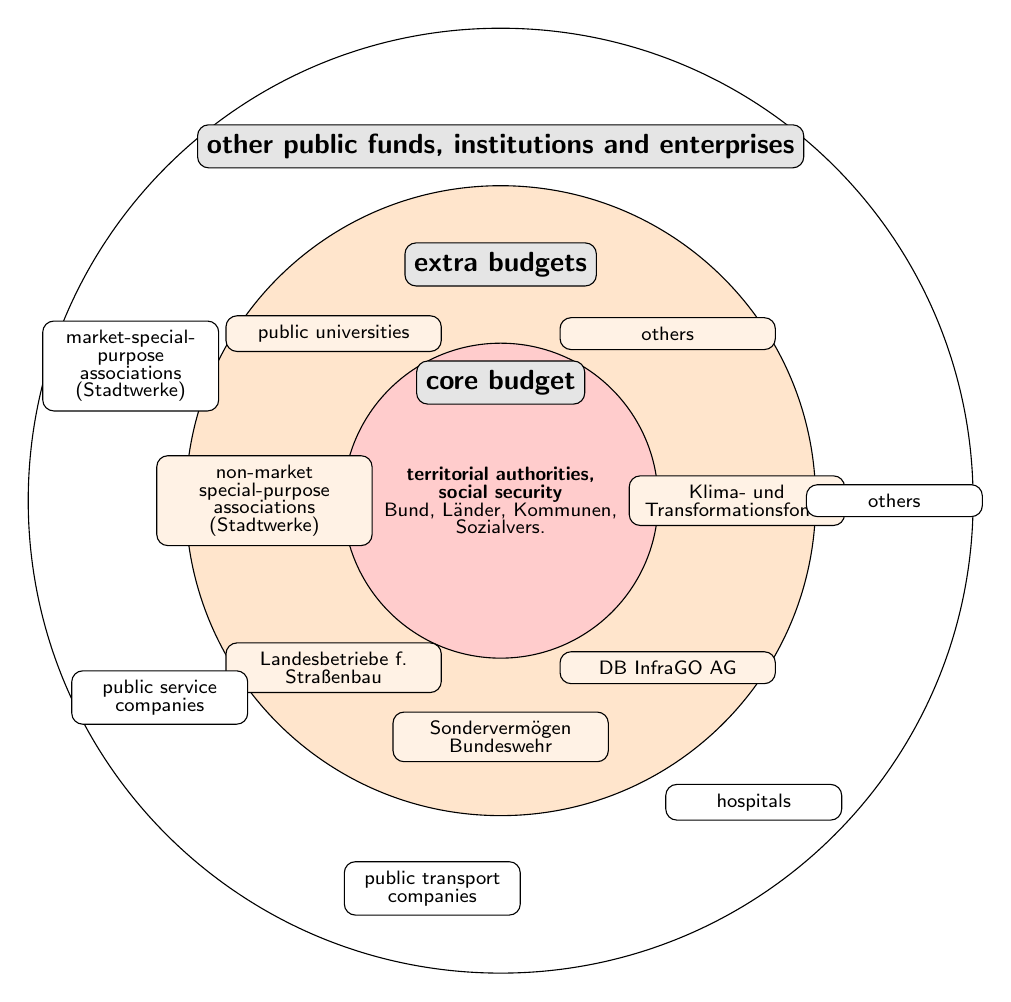
\begin{tikzpicture}
\renewcommand{\baselinestretch}{0.8}
    \tikzset{
        every node/.style={font=\sffamily\scriptsize}
    }
    \foreach [count=\i] \myshell/\mycolor in {other public funds{,} institutions and enterprises/white, extra budgets/orange, core budget/red}
    {
        \draw[fill=\mycolor!20] (0:0) circle (8-2*\i);
        \node[draw, rounded corners, fill=gray!20] at (90:6-1.5*\i) {\normalsize \textbf{\myshell}};
    }
    \node at (0,0) {
        \parbox{3cm}{
        \centering
        \textbf{territorial authorities, social security}\\
        Bund, Länder, Kommunen, Sozialvers.
        }
    };
    \foreach[count=\i] \myposten in {
        public universities, non-market special-purpose associations (Stadtwerke), Landesbetriebe f. Straßenbau, Sondervermögen Bundeswehr, DB InfraGO AG, Klima- und Transformationsfonds, others}
        {
        \node[draw,fill=orange!10,rounded corners] at (\i*45+90:8-5) {
            \parbox{2.5cm}{\centering
            \myposten
            }
        };
        }
    \foreach[count=\i] \myposten in {market-special-purpose associations (Stadtwerke), public service companies, public transport companies, hospitals, others}
        {
        \node[draw,fill=white,rounded corners] at (\i*50+110:8-3) {
            \parbox{2cm}{\centering
            \myposten
            }
        };
        }
\end{tikzpicture}
\end{document}